\documentclass[12pt,letterpaper]{article}
\usepackage[spanish]{babel}
\usepackage[utf8]{inputenc}
\usepackage{fancyhdr}
\usepackage{amsmath}
\usepackage{amsfonts}
\usepackage{amssymb}
\usepackage{float}
\usepackage{graphicx}
\author{Irarrázabal Callejas Norton John\\Norton.Dante.I@gmail.com\\Facultad de Ciencias\\Universidad de La Serena}
\title{Documentacion - desarrollador arbol AVL }
\date{}
\usepackage{listings}
\usepackage{multicol}
\usepackage[right=2cm,left=3cm,top=2cm,bottom=2cm,headsep=0cm,footskip=0.5cm]{geometry}
%-------------------------------------------------------------------------
\begin{document}
\maketitle
\begin{figure} [H]
\begin {center}
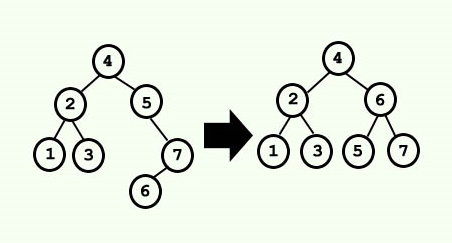
\includegraphics[width=10cm,height=5cm]{imagenavl} 
\end {center}
\end{figure}
%-------------------------------------------------------------------------
\newpage
\tableofcontents
%-------------------------------------------------------------------------
\newpage
\section{Análisis del arbol AVL}
\vskip 0.4cm
Definición. Un árbol AVL es un árbol binario de búsqueda que cumple con la condición de que la diferencia entre las alturas de los subárboles de cada uno de sus nodos es, como mucho 1, es decir balanceado.
\vskip 0.4cm
Recordamos que un árbol binario de busqueda consiste en que cada nodo cumple con que todos los nodos de su subárbol izquierdo son menores que la raíz y todos los nodos del subárbol derecho son mayores que la raíz.
\vskip 0.4cm
El tiempo de las operaciones sobre un árbol binario de búsqueda son O(log n) promedio, pero el peor caso es O(n), donde n es el número de
elementos.
\vskip 0.4cm
La propiedad de equilibrio que debe cumplir un árbol para ser AVL asegura que la profundidad del árbol sea O(log(n)), por lo que las operaciones sobre estas estructuras no deberán recorrer mucho para hallar el elemento deseado. 
\vskip 0.4cm
El tiempo de ejecución de las operaciónes sobre estos árboles es, a lo sumo O(log(n)) en el peor caso, donde n es la cantidad de elementos del árbol. Sin embargo, y como era de esperarse, esta misma propiedad de equilibrio de los árboles AVL implica una dificultad a la hora de insertar o eliminar elementos. Ya que es probable que estas operaciones afecten la propiedad de equilibrio.
\vskip 0.4cm
Por lo que se efectuan operaciones sobre el arbol conocidas como rotaciones, que nos ayudan a conservar el órden y a restaurar la propiedad de equilibrio de el arbol AVL.
\vskip 0.4cm 
$Factor$ $de$ $equilibrio$ $o$ $propiedad$ $de$ $equilibrio:$ $FE$ $=$ $altura$ $subarbol$ $derecho$ $-$ $altura$ $sub$ $arbol$ $izquierdo$.
\vskip 0.4cm 
Se usan 4 tipos de rotaciones.
\begin{itemize}
\item Rotacion Simple a la derecha: Se usa cuando el subarbol izquierdo de un nodo sea 2 unidades mas alto que el derecho, es decir que este cargado a la izquierda.FE (= -2)
\item Rotacion Simple a la izquierda: Se usa cuando subarbol derecho de un nodo sea 2 unidades mas alto que el izquierdo, es decir que este cargado a la derecha. (FE=2)
\item Rotacion Doble a la derecha:   Si FE$>$1 y su hijo derecho tiene signo -. Esto es el equivalente a 
i: aplicar rotacion simple a la derecha. ii: aplicar rotacion simple a la izquierda.
\item Rotacion Doble a la izquierda: Si FE$<$-1 y su hijo izquierdo tiene signo +.
i: aplicar rotacion simple a la izquierda. ii: aplicar rotacion simple a la derecha.
\end{itemize}
%-------------------------------------------------------------------------
\newpage
\section{Ejemplos}
\vskip 1.3cm
\begin{multicols}{2}
\begin{flushleft}
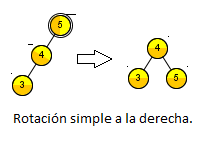
\includegraphics[width=6cm,height=5cm]{rotacionsimplederecha} 
\vskip 3.6cm
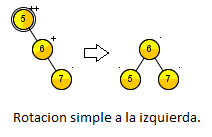
\includegraphics[width=6cm,height=5cm]{rotacionsimpleizquierda} 
\end{flushleft}

\begin{flushright}
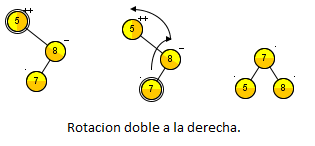
\includegraphics[width=8cm,height=5cm]{rotaciondoblederecha} 
\vskip 3.6cm
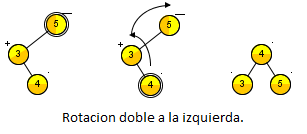
\includegraphics[width=8cm,height=5cm]{rotaciondobleizquierda} 
\end{flushright}

\end{multicols}
%-------------------------------------------------------------------------
\newpage
\section{Implementación arbol AVL}
El arbol avl se elaboro en Eclipse Jee Oxygen es una plataforma de software compuesto por un conjunto de herramientas de programación de código abierto multiplataforma para desarrolladores java.
\vskip 0.6cm
Pueden existir diversas formas de implementar un arbol AVL. Sin embargo, la implementación que yo hice para los nodos del arbol AVL es la siquiente:
\vskip 0.8cm
\begin{lstlisting}
public class Nodo_arbol_AVL {
	int Valor, FE;
	Nodo_arbol_AVL hijoizquierdo,hijoderecho;
	
	public Nodo_arbol_AVL (int Valor1) {
		this.Valor=Valor1;
		this.FE=0;
		this.hijoizquierdo=null;
		this.hijoderecho=null;
	}
}
\end{lstlisting}
\vskip 0.6cm
Los nodos pueden tener muchos mas datos ya sean String, int, double etc. Sin embargo por simplicidad solo usaremos un dato de tipo entero, ahora si lo queremos con mas datos bastaria con incoporar otra variable.
\vskip 0.6cm
Cada nodo tendra su propio factor de equilibrio, para poder evaluar el balance del arbol AVL. Ademas de un hijo izquierdo y un hijo derecho de su misma clase.
\vskip 0.8cm
Ahora el arbol AVL lo defini como API\_AVL y este tendra solamente el nodo raiz.
\begin{lstlisting}
public class API_AVL{
	private Nodo_arbol_AVL raiz;
	
	public API_AVL() {
		raiz=null;
	}
}
\end{lstlisting}
\vskip 0.8cm
Ahora recordemos que cada una de estas clases tiene múltiples metodos sin embargo no es menester nombrarlos todos en este documento, para esta causa incorpore diagramas UML y el Javadoc en donde podran encontrar todos los metodos.
%-------------------------------------------------------------------------
\newpage
\begin{thebibliography}{10}
\bibitem{}{Árboles AVL: rua.ua.es/dspace/handle/10045/16037}
\end{thebibliography}
\end{document}